\documentclass{article}
\usepackage[utf8]{inputenc}
\usepackage[margin=2cm]{geometry}
\usepackage[spanish]{babel}
\usepackage{graphicx}
\usepackage{lipsum}
\usepackage{amsmath, physics}
\usepackage{authblk}
\usepackage{makecell, array}
\usepackage[square,numbers]{natbib}
\usepackage{float}
\usepackage{gensymb}
\usepackage{url}
\usepackage{multirow}
\usepackage{hhline}
\usepackage{caption}

\renewcommand{\tablename}{Figura}
\renewcommand{\figurename}{Figura}
\AtBeginDocument{\renewcommand\tablename{Figura}}
\AtBeginDocument{\renewcommand\figurename{Figura}}

\providecommand{\keywords}[1]
{
	\small
	\textbf{\textit{Keywords---}} #1
}

\providecommand{\palabrasclave}[1]
{
	\small
	\textbf{\textit{Palabras Clave---}} #1
}

\makeatletter 
\let\c@table\c@figure
\makeatother

\title{Circuitos Básicos}
\author{
	{Anderson Stib Ibarra Orozco$^{1}$, Juan Jose Medina Velasquez$^{2}$}
	\small{\texttt{$^{1}$asibarrao,$^{2}$jjmedinav}}\\
	\small{Universidad Nacional de Colombia}	
}
\date{\today}

 \begin{document}
 \twocolumn[
	   \begin{@twocolumnfalse}
	        \maketitle
	        \vspace*{-1cm}
	        \begin{center}
	    	    \rule{0.9\textwidth}{0.1mm}
    	    \end{center}
            \selectlanguage{spanish}
    	    \begin{abstract}
		        
	    	    \vspace*{0.5cm}
	        \end{abstract}
	        \palabrasclave{Emisión termoiónica, Ley de Richardson-Dushman, Tungsteno}
	    \end{@twocolumnfalse}
	    \begin{center}
		    \rule{0.9\textwidth}{0.1mm}
	    \end{center}	
	    \vspace*{0.5cm}
	]

 \section{Marco teórico}
 Ley de ohm.
 leyes de Kirchoff.
 
 \section{Procedimiento}
 Para realizar el experimento se utilizó el circuito mostrado en la figura \ref{fig:circuito}.
 
 \begin{figure}[H]
 \centering
 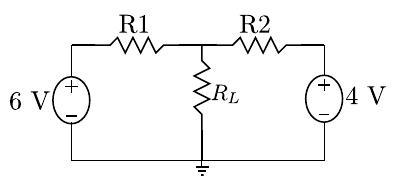
\includegraphics[width=0.5\textwidth]{fig/circuito.jpg}
 \caption{circuito utilizado en el experimento}
 \label{fig:circuito}
 \end{figure}
 
 Para la primera parte del experimento se tomaron los valores medidos de los voltajes de las fuentes y de las resistencias, con los cuales se procediò a utilizar las leyes de Kirchoff y la ley de Ohm para encontrar las corrientes y los voltajes de cada una de las resistencias   
 
 \section{Análisis de resultados}
 \section{conclusiones}
 \end{document}